\section{Análisis del sistema}
\par En esta sección se detallará el análisis del sistema sobre el que se basará el proyecto, dividido en las siguientes partes:
\begin{itemize}
	\item \textbf{Sistema Operativo:} sistema operativo donde se utilizará el software.
	\item \textbf{Software: }esta parte incluye tanto el software a desarrollar como la plataforma sobre la que se desarrollará.
	\item \textbf{Hardware: }el hardware necesario para los dos apartados anteriores. 
\end{itemize}

\subsection{Sistema Operativo}
\par Como sistema operativo se utilizará Linux, concretamente RHEL 7.4 dado que de esa forma se tendrá acceso al soporte de Red Hat 24/7. Esto implica un gasto adicional por parte del cliente, pero en el caso de que no esté dispuesto a asumirlo se utilizará Debian 9.
\par Ambos sistemas operativos han sido escogidos por las siguientes características:
\begin{itemize}
	\item \textbf{Fiabilidad:} tanto RHEL 7.4 como Debian 9 son \textit{distribuciones} de Linux, con una filosofía y configuración especializada en construir un sistema estable, haciéndolo idóneo para servidores que requieren estar 24/365 activos.
	\item \textbf{Ligereza:} dada la naturaleza de Linux, el sistema es más ligero que Windows Server. Escogiendo Linux frente a Windows Server, disponemos de más recursos del sistema para asignarlos al software.
	\item \textbf{Seguridad:} Linux en servidores es igual o más seguro que Windows Server, añadiendo además una capa adicional de seguridad mediante la encapsulación de servicios en \textit{intancias / contenedores} virtuales.
	\item \textbf{Virtualización avanzada:} en Linux es posible virtualizar los servicios del software, por lo que un mismo servidor de Linux puede contener varias instancias del software a desplegar listas de forma casi instantánea y de forma individual, por lo que en el caso de que una instancia virtualizada se comprometiese no afectaría al resto.
\end{itemize}
\subsection{Software}
\par A petición del cliente, se utilizará Liferay EE 7 como portal web. Esta solución software está creada y desarrollada de forma comunitaria, pero se puede adquirir un soporte adicional profesional. La adquisición de dicho soporte está recomendada pero dependerá de la decisión del cliente el si adquirirlo o no dado que incrementa los costes del proyecto (sobre todo a largo plazo).
\par La aplicación web está desarrollada en Java y soporta la última versión estable de Java, que es Java EE 8.

\subsection{Hardware}
\par Dada la naturaleza de Java, el fabricante de Liferay recomienda los siguientes requisitos para el servidor:
\begin{itemize}
	\item \textbf{CPU:} 16 cores.
	\item \textbf{RAM:} 16 GB.
	\item \textbf{DISCO:} al menos 500GB.
\end{itemize}
\par Este sistema valdría para 1000-2000 usuarios concurrentes con una tasa de 85 transacciones / segundo. La recomendación del fabricante para un sistema que soporte esa cantidad de usuarios o mayor sería la siguiente:

\begin{figure}
  \centering
    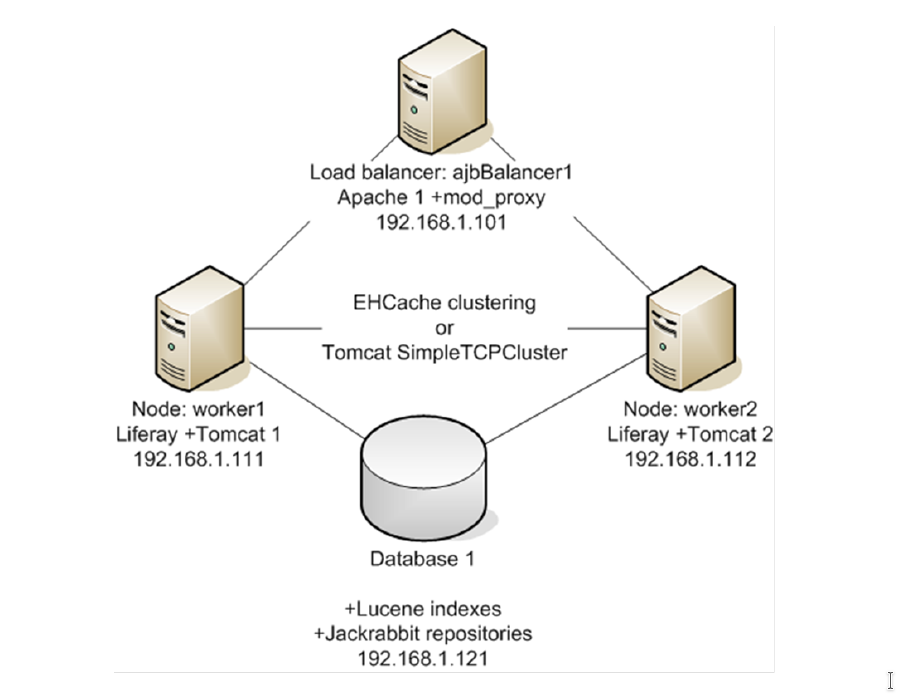
\includegraphics[width=0.5\textwidth]{./img/systemstructure.png}
  \caption{Estructura de los servidores.}
  \label{fig:systemstructure}
\end{figure}
Figure \ref{fig:systemstructure} Diagrama del sistema.

\par Con cada servidor de Liferay teniendo la mitad de requisitos especificados anteriormente.